\section{Results and Discussion}
\label{sec:fn_opt:results}

    This section presents optimization results for 20 classical functions using three selection strategies: Random, 
    Tournament, and Roulette. Detailed tables and figures offer insights into the time efficiency and effectiveness of 
    each evolutionary phase, along with the final optimization outcomes.

    Analysis reveals the Tournament Selector's superior performance compared to the Random and Roulette Selectors, as 
    shown in \vref{fig:fn_opt:results:cross_in_tray}. The Random and Roulette selectors produce similar results, 
    attributed to the Roulette Selector's probabilistic nature, akin to a weighted Random Selector. As evolution 
    progresses, the differences in fitness weights among individuals decrease, making the Roulette Selector's behavior 
    more like the Random Selector's.
    
    Both Random and Roulette selectors can occasionally find the global optimum but struggle to consistently retain it. 
    In contrast, the Tournament Selector, thanks to its competitive approach, not only finds but also maintains optimal 
    solutions effectively. This observation suggests that a target fitness criterion might be more fitting than a 
    stagnation termination criterion for the Random and Roulette selectors, as they lack the ability to sustain the 
    optimal solution over time. A target fitness criterion (natively supported by our framework) may be more appropriate
    for these selectors, as it would allow them to terminate once the optimal solution is found, rather than continuing
    to run until the maximum generation limit is reached.
    
    The analysis utilized the \texttt{EvolutionPlotter} listener for generating these figures, a feature not readily 
    available in other frameworks, highlighting the unique capabilities of the presented framework.

    \begin{figure}[ht!]
        \centering
        \begin{subfigure}{.45\textwidth}
            \centering  
            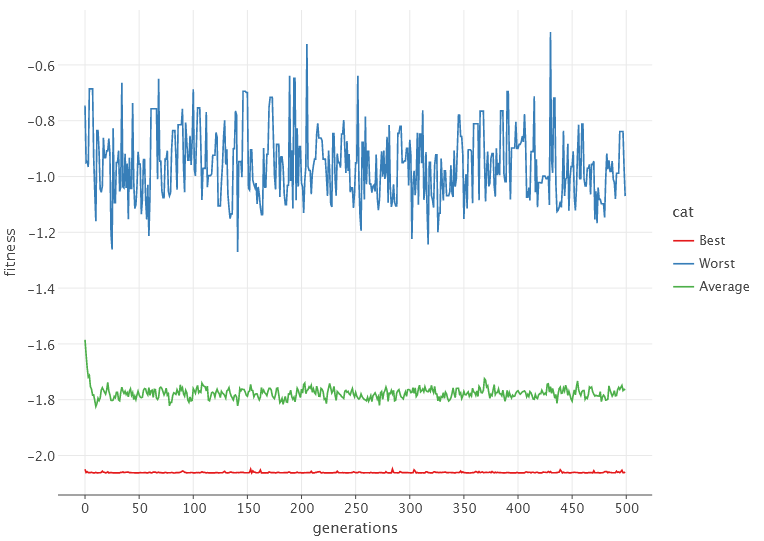
\includegraphics[width=\linewidth]{img/cross_in_tray_random.png}
            \caption{Random Selector}
        \end{subfigure}
        \begin{subfigure}{.45\textwidth}
            \centering
            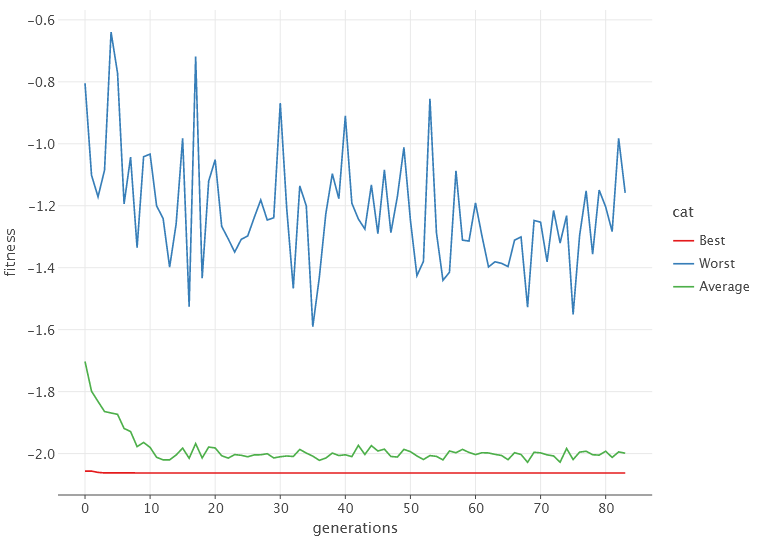
\includegraphics[width=\linewidth]{img/cross_in_tray_tournament.png}
            \caption{Tournament Selector}
        \end{subfigure}
        \begin{subfigure}{.45\textwidth}
            \centering
            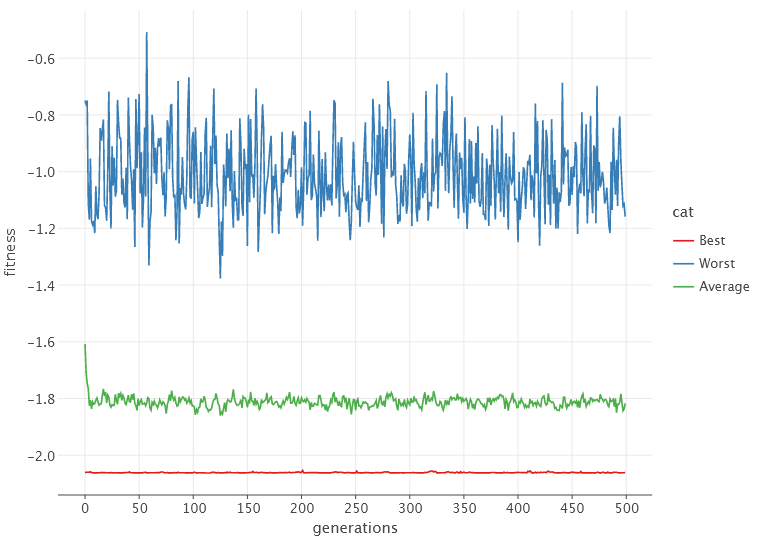
\includegraphics[width=\linewidth]{img/cross_in_tray_roulette.png}
            \caption{Roulette Selector}
        \end{subfigure}
        \caption{Fitness evolution for the Cross-in-tray function under different selection strategies.}
        \label{fig:fn_opt:results:cross_in_tray}
    \end{figure}

    We now detail the optimization results for each selector across he various functions. To mitigate JVM warmup effects, each experiment was conducted four times, with the initial run excluded from analysis. The reported 
    results represent the average of the subsequent three iterations, focusing primarily on the consistency of 
    execution times, as fitness values heavily depend on the chosen operators. Due to the unique nature of our solution 
    (as discussed in the previous section), a direct comparison with other frameworks is not feasible. This results are provided in \vref{app:fn_opt:results}.

    Analysis shows minimal variation in selection times across all selectors, indicating consistent performance. The 
    Random Selector, requiring minimal computational effort, shows the lowest average selection time. The Tournament 
    and Roulette selectors have similar times, with the Roulette Selector slightly lagging due to the additional 
    computational work involved in calculating individual fitness weights.
    
    Average evolution times are comparably close across selectors, roughly within the \(10^{-1}\) second range. The 
    Tournament Selector slightly leads in speed, attributed to its efficiency in maintaining optimal solutions without 
    needing to explore every generation. Conversely, the Roulette Selector is somewhat slower than the Random Selector, 
    burdened by the extra computational effort for fitness weight calculations.
    
    The Tournament Selector stands out by stopping the evolutionary process before reaching the maximum generation 
    limit, thereby demonstrating its efficiency in sustaining optimal solutions. It consistently achieves the lowest 
    average error, signifying its effectiveness in identifying optimal solutions. The Roulette and Random selectors 
    show comparable average errors, with the Roulette Selector marginally better, suggesting more consistent 
    performance.
    
    Exceptions to the Tournament Selector's performance are noted in functions like Rastrigin, Egg Holder, and 
    Schaffer, where multiple local optima challenge the algorithm's escape capabilities. However, for functions like 
    Booth with a clearer path to the global optimum, the Tournament Selector shows strong performance.

    This analysis underscores the Tournament Selector's robustness and the importance of strategic selection criteria 
    based on an algorithm's ability to sustain optimal solutions.

    A key challenge with our problem and solution is that they aren't readily addressed by the frameworks discussed 
    in this thesis. The issue stems from our need for unique ranges for each gene, a feature not directly available 
    in these frameworks. While it's possible to adapt other frameworks to meet this requirement, doing so would 
    demand considerable customization to achieve the desired functionality.

    For example, implementing the solution in \textit{Jenetics} would require the creation of a custom class to
    simulate the behavior of double-valued genes with different ranges. Additionally, we'd need to define classes 
    for the various optimization functions, potentially utilizing \textit{functional interfaces}. The core of the 
    solution involves creating a class that inherits from the \texttt{Problem} interface, necessitating the 
    definition of \texttt{fitness} and \texttt{codec} methods. The \texttt{fitness} method calculates the fitness 
    for a genotype, while the \texttt{codec} method generates a \texttt{Codec} using the custom class, facilitating 
    the creation of \texttt{Genotype} instances. This \texttt{Codec} is essential for configuring the GA 
    \texttt{Engine} to execute the genetic algorithm.

    For \textit{DEAP}, adapting the solution might be somewhat simpler. A custom crossover function would be needed 
    for the average crossover, and another for the random mutation, but the existing \textit{gaussian mutation} 
    operator could be suitable for our problem, perhaps with minor adjustments. This reduces the complexity 
    compared to \textit{Jenetics}, but still demands a thorough understanding of \textit{DEAP} and some 
    customization.

    Adapting both examples to the frameworks would necessitate thorough expertise in their use and considerable 
    effort. Additionally, the available documentation for these frameworks may not be comprehensive enough, 
    potentially leading to a need for extensive experimentation to achieve the desired implementation.

    The solution's implementation showcases the ease of adapting to various optimization functions, selection 
    strategies, mutation and crossover operators, and termination criteria, thanks to the framework's modular 
    architecture. This flexibility is \vref{code:fn_opt:sol:engine}, where The creation of the engine is abstracted to
    a single function, allowing for easy reuse across different optimization functions.The framework's comprehensive 
    set of features eliminates the need for custom operations or structures. Additionally, Kotlin's support for 
    functions as first-class citizens simplifies defining fitness functions without extra interfaces or classes, a 
    capability also present in languages like Scala or Python. Another key aspect is the already mentioned capability of
    the framework to create genes tailored to specific search spaces, enhancing its versatility in addressing diverse
    optimization tasks. As a final remark, the ability to visualize the fitness evolution of the population is a
    valuable feature for debugging and analysis, not readily available in other frameworks.